\chapter[METODOLOGI PENELITIAN]{\\ METODOLOGI PENELITIAN}
Metodologi yang diterapkan pada penelitian menjadi pokok bahasan pada bab ini. Alur perencanaan penelitian, pengumpulan dan analisis data, serta hasil penelitian akan dijelaskan secara terperinci. Sebagai tambahan, penjelasan dalam bab ini juga meliputi komponen-komponen lain seperti pendekatan penelitian, teknik pengumpulan data, jenis data yang terkumpul, metode analisis, dan instrumen pendukung yang digunakan.

\section{Tahapan Penelitian}
\lipsum[1]

\section{Penjelasan Tahapan Penelitian 1}
\lipsum[1]

\subsection{Sub Penjelasan Tahapan Penelitian 1}
\lipsum[1]2

\begin{figure}[H]
    \centering
    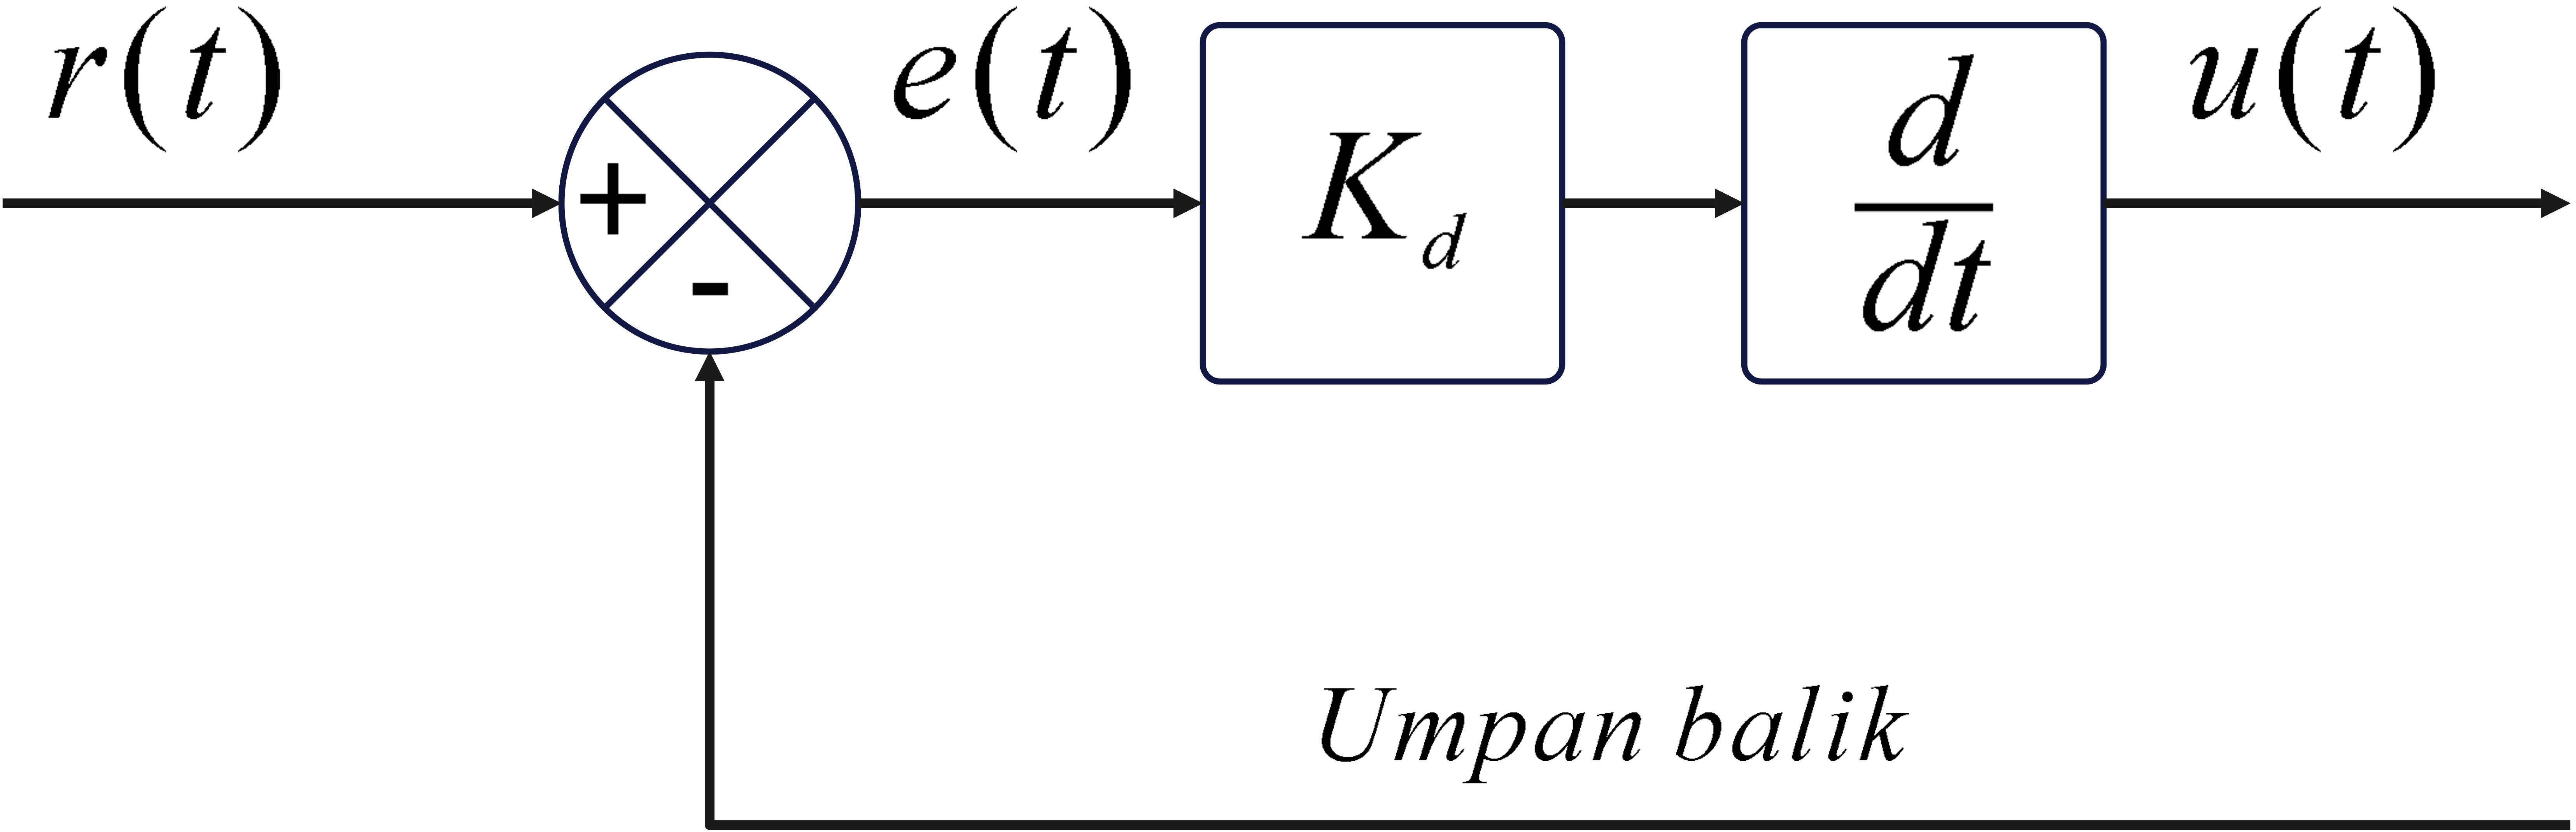
\includegraphics[width=0.8\linewidth]{images/diagram.png}
    \caption{Contoh gambar 1}
    \label{gambar1}
\end{figure}

\lipsum[1]

\subsection{Sub Penjelasan Tahapan Penelitian 1}
\lipsum[1]

\section{Penjelasan Tahapan Penelitian 2}
\lipsum[1]

\subsection{Sub Penjelasan Tahapan Penelitian 2}
\lipsum[1]

\lipsum[1]